% \documentclass[table]{beamer}
\documentclass[table,handout]{beamer}
\setbeameroption{show notes}
% \setbeameroption{hide notes}
% \setbeameroption{show only notes}
\usepackage{varwidth}

\newif\ifhide
\newif\ifpost
\newif\ifhideclicker

% \hidetrue
% \hideclickertrue
% \posttrue

\newcommand{\whiteout}[1]{\textcolor{white}{#1}}
% \newcommand{\whiteoutbox}[1]{\fcolorbox{white}{white}{\parbox{\dimexpr \linewidth-2\fboxsep-2\fboxrule}{\whiteout{#1}}}}
% \newcommand{\notebox}[1]{\fcolorbox{blue}{white}{\parbox{\dimexpr \linewidth-2\fboxsep-2\fboxrule}{#1}}}
\newcommand{\whiteoutbox}[1]{\fcolorbox{white}{white}{\parbox{\linewidth}{\whiteout{#1}}}}
\newcommand{\notebox}[1]{\fcolorbox{blue}{white}{\parbox{\linewidth}{#1}}}
\newcommand{\blankbox}[1]{\phantom{\varwidth{\linewidth}\whiteoutbox{#1}\endvarwidth}}
\newcommand{\blank}[1]{\phantom{\varwidth{\linewidth}#1\endvarwidth}}

\ifhide%
    \newcommand{\hmask}[1]{\blank{#1}}%
\else%
    \newcommand{\hmask}[1]{#1}%
\fi

\ifhide%
    \newcommand{\wout}[1]{\whiteout{#1}}%
\else%
    \newcommand{\wout}[1]{#1}%
\fi

\ifhide%
    \newcommand{\hignore}[1]{}%
\else%
    \newcommand{\hignore}[1]{#1}%
\fi

\ifpost%
    \newcommand{\nopost}[1]{}%
\else%
    \newcommand{\nopost}[1]{#1}%
\fi

\ifhideclicker%
    \newcommand{\clickerslide}[1]{\stepcounter{clickerQuestionCounter}%
        \begin{frame}[t]
            \textcolor{blue}{Q \arabic{clickerQuestionCounter}:}
        \end{frame}}
\else%
    \newcommand{\clickerslide}[1]{#1}%
\fi

\ifhide%
    \newcommand{\hidebox}[1]{\blank{#1}}%
\else%
    \newcommand{\hidebox}[1]{\notebox{#1}}%
\fi

\ifhide%
    \newcommand{\wbox}[1]{\whiteoutbox{#1}}%
\else%
    \newcommand{\wbox}[1]{\notebox{#1}}%
\fi

\ifhide%
    \newcommand{\nbox}[1]{\blankbox{#1}}%
\else%
    \newcommand{\nbox}[1]{\notebox{#1}}%
\fi

\ifhideclicker%
    \newcommand{\clickeranswer}[1]{#1}%
\else%
    \ifhide%
        \newcommand{\clickeranswer}[1]{#1}%
    \else%
        \newcommand{\clickeranswer}[1]{\textbf{\textcolor{blue}{#1}}}%
    \fi
\fi

\usepackage{beamerthemesplit}
% \usetheme{boxes}
\usetheme{Malmoe}
\usecolortheme{seahorse}
% \usecolortheme{seagull}
\usepackage{ifthen}
\usepackage{xspace}
\usepackage{multirow}
\usepackage{multicol}
\usepackage{booktabs}
\usepackage{xcolor}
\usepackage{wasysym}
\usepackage{comment}
\usepackage{hyperref}
\hypersetup{pdfborder={0 0 0}, colorlinks=true, urlcolor=blue, linkcolor=blue, citecolor=blue}
\usepackage{changepage}
\usepackage[compatibility=false]{caption}
\captionsetup[figure]{font=scriptsize, labelformat=empty, textformat=simple, justification=centering, skip=2pt}
\usepackage{tikz}
\usetikzlibrary{trees,calc,backgrounds}

\usepackage[bibstyle=joaks-slides,maxcitenames=3,mincitenames=1,backend=biber]{biblatex}

\newrobustcmd*{\shortfullcite}{\AtNextCite{\renewbibmacro{title}{}\renewbibmacro{in:}{}\renewbibmacro{number}{}}\fullcite}

\newrobustcmd*{\footlessfullcite}{\AtNextCite{\renewbibmacro{title}{}\renewbibmacro{in:}{}}\footfullcite}

% Make all footnotes smaller
% \renewcommand{\footnotesize}{\scriptsize}

\definecolor{myGray}{gray}{0.9}
\colorlet{rowred}{red!30!white}

\setbeamertemplate{blocks}[rounded][shadow=true]

\setbeamercolor{defaultcolor}{bg=structure!30!normal text.bg,fg=black}
\setbeamercolor{block body}{bg=structure!30!normal text.bg,fg=black}
\setbeamercolor{block title}{bg=structure!50!normal text.bg,fg=black}

\newenvironment<>{varblock}[2][\textwidth]{%
  \setlength{\textwidth}{#1}
  \begin{actionenv}#3%
    \def\insertblocktitle{#2}%
    \par%
    \usebeamertemplate{block begin}}
  {\par%
    \usebeamertemplate{block end}%
  \end{actionenv}}

\newenvironment{displaybox}[1][\textwidth]
{
    \centerline\bgroup\hfill
    \begin{beamerboxesrounded}[lower=defaultcolor,shadow=true,width=#1]{}
}
{
    \end{beamerboxesrounded}\hfill\egroup
}

\newenvironment{onlinebox}[1][4cm]
{
    \newbox\mybox
    \newdimen\myboxht
    \setbox\mybox\hbox\bgroup%
        \begin{beamerboxesrounded}[lower=defaultcolor,shadow=true,width=#1]{}
    \centering
}
{
    \end{beamerboxesrounded}\egroup
    \myboxht\ht\mybox
    \raisebox{-0.25\myboxht}{\usebox\mybox}\hspace{2pt}
}

\newenvironment{mydescription}{
    \begin{description}
        \setlength{\leftskip}{-1.5cm}}
    {\end{description}}

\newenvironment{myitemize}{
    \begin{itemize}
        \setlength{\leftskip}{-.3cm}}
    {\end{itemize}}

% footnote without a marker
\newcommand\barefootnote[1]{%
  \begingroup
  \renewcommand\thefootnote{}\footnote{#1}%
  \addtocounter{footnote}{-1}%
  \endgroup
}

% define formatting for footer
\newcommand{\myfootline}{%
    {\it
    \insertshorttitle
    \hspace*{\fill} 
    \insertshortauthor, \insertshortinstitute
    % \ifx\insertsubtitle\@empty\else, \insertshortsubtitle\fi
    \hspace*{\fill}
    \insertframenumber/\inserttotalframenumber}}

% set up footer
\setbeamertemplate{footline}{%
    \usebeamerfont{structure}
    \begin{beamercolorbox}[wd=\paperwidth,ht=2.25ex,dp=1ex]{frametitle}%
        % \Tiny\hspace*{4mm}\myfootline\hspace{4mm}
        \tiny\hspace*{4mm}\myfootline\hspace{4mm}
    \end{beamercolorbox}}

% remove navigation bar
\beamertemplatenavigationsymbolsempty

\makeatletter
    \newenvironment{noheadline}{
        \setbeamertemplate{headline}[default]
        \def\beamer@entrycode{\vspace*{-\headheight}}
    }{}
\makeatother

\newcounter{clickerQuestionCounter}
\ifhideclicker%
\newenvironment{clickerquestion}
{ \stepcounter{clickerQuestionCounter}
  \begin{enumerate}[Q \arabic{clickerQuestionCounter}:]\color{white} }
{ \end{enumerate} }
\else%
\newenvironment{clickerquestion}
{ \stepcounter{clickerQuestionCounter}
  \begin{enumerate}[Q \arabic{clickerQuestionCounter}:] }
{ \end{enumerate} }
\fi

\ifhideclicker%
\newenvironment{clickeroptions}
{ \begin{enumerate}[\begingroup\color{white} 1)\endgroup]\color{white} }
{ \end{enumerate} }
\else%
\newenvironment{clickeroptions}
{ \begin{enumerate}[\begingroup\color{red} 1)\endgroup] }
{ \end{enumerate} }
\fi


\tikzstyle{centered} = [align=center, text centered, font=\sffamily\bfseries]
\tikzstyle{skip} = [centered, inner sep=0pt, fill]
\tikzstyle{empty} = [centered, inner sep=0pt]
\tikzstyle{inode} = [centered, circle, minimum width=4pt, fill=black, inner sep=0pt]
\tikzstyle{tnode} = [centered, circle, inner sep=1pt]
\tikzset{
  % edge styles
  level distance=10mm,
  mate/.style={edge from parent/.style={draw,distance=3pt}},
  mleft/.style={grow=left, level distance=10mm, edge from parent path={(\tikzparentnode.west)--(\tikzchildnode.east)}},
  mright/.style={grow=right, level distance=10mm, edge from parent path={(\tikzparentnode.east)--(\tikzchildnode.west)}},
  % node styles
  male/.style={rectangle,minimum size=4mm,fill=gray!80},
  female/.style={circle,minimum size=4mm,fill=gray!80},
  amale/.style={male,fill=red},
  afemale/.style={female,fill=red},
}

\newcommand{\highlight}[1]{\textcolor{violet}{\textit{\textbf{#1}}}}
\newcommand{\super}[1]{\ensuremath{^{\textrm{\sffamily #1}}}}
\newcommand{\sub}[1]{\ensuremath{_{\textrm{\sffamily #1}}}}
\newcommand{\dC}{\ensuremath{^\circ{\textrm{C}}}}
\newcommand{\tb}{\hspace{2em}}
\providecommand{\e}[1]{\ensuremath{\times 10^{#1}}}
\newcommand{\myHangIndent}{\hangindent=5mm}

\newcommand{\spp}[1]{\textit{#1}}

\newcommand\mybullet{\leavevmode%
\usebeamertemplate{itemize item}\hspace{.5em}}

\makeatletter
\newcommand*{\rom}[1]{\expandafter\@slowromancap\romannumeral #1@}
\makeatother

\newcommand{\blankslide}{{\setbeamercolor{background canvas}{bg=black}
\setbeamercolor{whitetext}{fg=white}
\begin{frame}<handout:0>[plain]
\end{frame}}}

\newcommand{\whiteslide}{
\begin{frame}<handout:0>[plain]
\end{frame}}

\newcommand{\f}[1]{\ensuremath{F_{#1}}}
\newcommand{\x}[1]{X\ensuremath{^{#1}}}
\newcommand{\y}[1]{Y\ensuremath{^{#1}}}

% Population growth macros
\newcommand{\popsize}[1]{\ensuremath{N_{#1}}}
\newcommand{\popgrowthratediscrete}[1]{\ensuremath{\lambda_{#1}}}
\newcommand{\popgrowthrate}[1]{\ensuremath{r_{#1}}}
\newcommand{\ptime}{\ensuremath{t}\xspace}

\tikzset{hide on/.code={\only<#1>{\color{white}}}}
\tikzset{
    invisible/.style={opacity=0},
    visible on/.style={alt={#1{}{invisible}}},
    alt/.code args={<#1>#2#3}{%
        \alt<#1>{\pgfkeysalso{#2}}{\pgfkeysalso{#3}}
        % \pgfkeysalso doesn't change the path
    },
}

\bibliography{../bib/references}
\author[J.\ Oaks]{
    %Jamie R.\ Oaks\inst{1}
    Jamie R.\ Oaks
}
\institute[BIOL 180]{
    \inst{}%
        BIOL 180: Introductory Biology
}



\title[Mendel: Monohybrid crosses]{Mendel: Monohybrid crosses}
% \date{\today}
\date{April 6, 2015}

\begin{document}

\begin{noheadline}
\maketitle
\end{noheadline}

\nopost{
\begin{noheadline}
\begin{frame}[c]
    \vspace{-6mm}
    \begin{center} 
        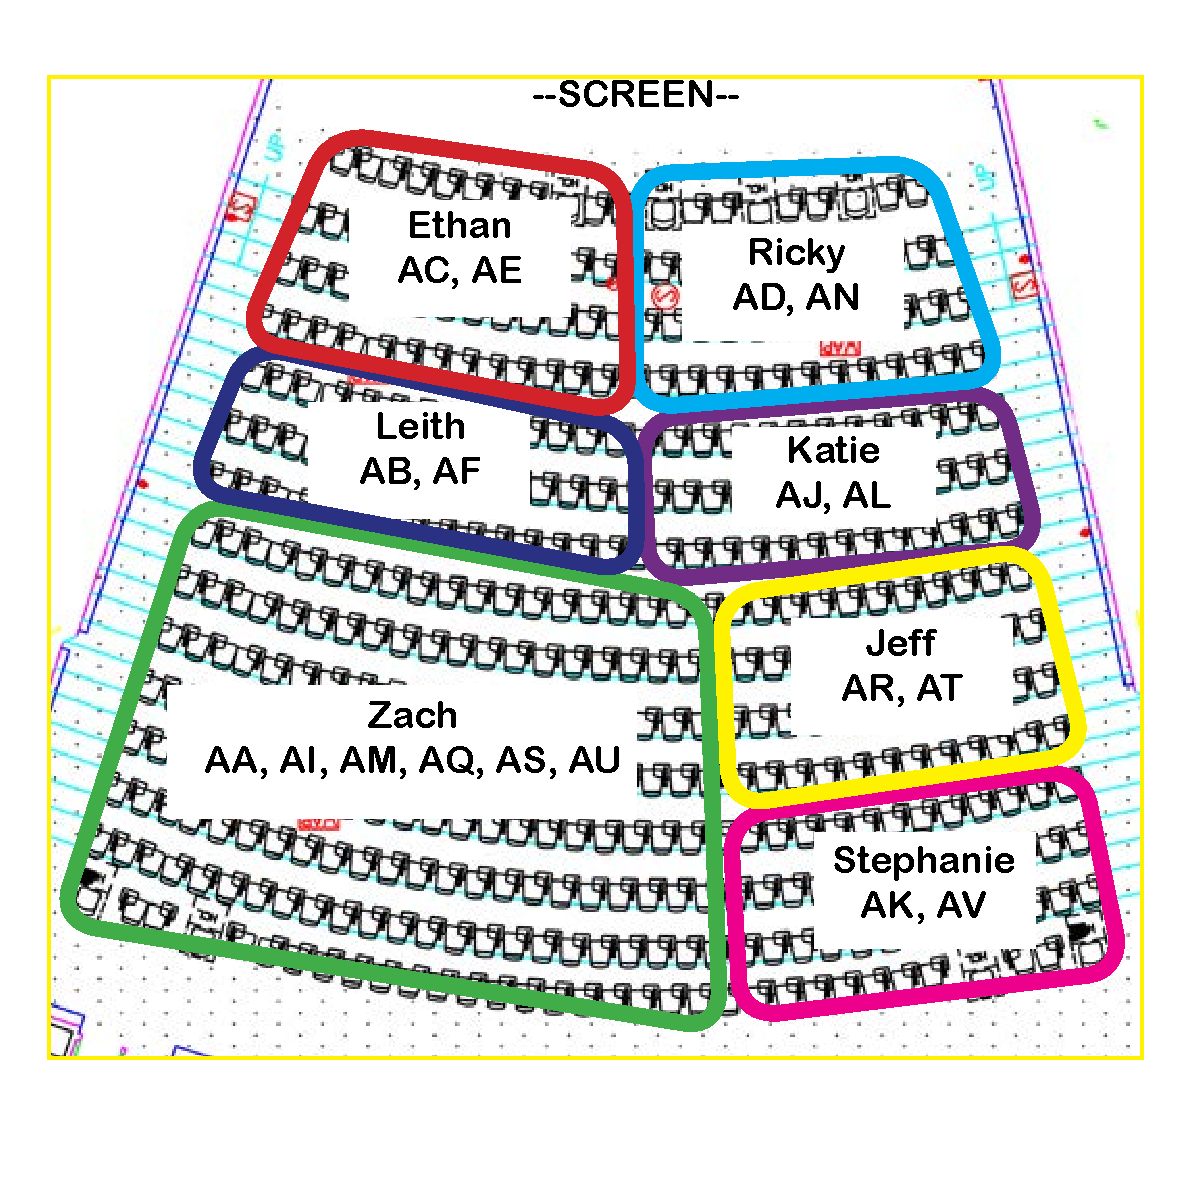
\includegraphics[height=1.3\textheight]{../images/seating-chart.pdf}
    \end{center}
\end{frame}
\end{noheadline}
}

\begin{noheadline}
\begin{frame}
    \begin{clickerquestion}
        \item If a Caucasian moves to the subtropics or tropics, her skin may
            respond to the increased ultraviolet light by tanning. Which of the
            following statements regarding this pattern is correct?
        \begin{clickeroptions}
            \item When a person's skin tans, they are adapting.
            \item \clickeranswer{When a person's skin tans, they are
                    acclimating.}
            \item The trait of being able to tan is an acclimation.
            \item \clickeranswer{The trait of being able to tan is an
                    adaptation.}
        \end{clickeroptions}
    \end{clickerquestion}
\end{frame}
\end{noheadline}

\begin{noheadline}
\begin{frame}
    \begin{clickerquestion}
        \item Which of the following best characterizes evolution by natural
            selection?
        \begin{clickeroptions}
            \item The strongest individuals in a population survive best and
                reproduce the most. Weak individuals are eliminated. 
            \item Survival of the fittest.
            \item \clickeranswer{Any population that exhibits heritable
                    variation and differential reproductive success will
                    evolve.}
            \item Adaptations are for the good of the species---they help the
                species survive.
        \end{clickeroptions}
    \end{clickerquestion}
\end{frame}
\end{noheadline}

\begin{noheadline}
\begin{frame}
\frametitle{Today's issues:}
\tableofcontents[subsectionstyle=hide]
\end{frame}
\end{noheadline}

\section{Darwin's dilemma}

\begin{frame}
    \frametitle{Darwin's dilemma: the problem of variation}

    \uncover<1->{
    The fact of evolution was accepted in the 1870s--1880s.
    }
    
    \bigskip

    \uncover<1->{
    Natural selction an evolutionary process was controversial until 1930s.
    }

    \begin{enumerate}
        \item<1-> Selection will exhaust variation; Why would this ``stop''
            evolution?
            \nbox{\scriptsize If certain traits are favored generation after
                generation, then soon only those certain traits will exist. No
                more variation---no more evolution (even if the environment
                changes)}
            % \vspace{2mm}
        \item<1-> Blending inheritance will eliminate new, advantageous
            variants; why would this ``stop'' evolution?
            \nbox{\scriptsize A new advantageous trait will be rare. It would
                blend after mating and not be pure in the next generation---it
                would be ``watered down.'' This would happen again and again,
                until the trait would disappear for all intents and purposes.}
    \end{enumerate}
\end{frame}

\section{Mendel's solution}

\begin{frame}
    \frametitle{Mendel's solution}

    \begin{itemize}
        \item<1-> Mendel was trying to understand the basic patterns of inheritance

        \item<2-> Two contrasting hypotheses:
            \begin{enumerate}
                \item<2-> Blending inheritance
                    \nbox{The genetic material from each parent mixes
                        together---blending to form intermediate phenotypes}

                \item<2-> Inheritance of acquired characters
                    \nbox{Traits of individuals change through use or exposure
                        to an environment; the changed form of the trait is is
                        passed on to offspring}
            \end{enumerate}

        \item<2-> What are these?
    \end{itemize}
\end{frame}

\section{Analyzing monohybrid crosses}

\subsection{Garden peas as a model organism}

\begin{frame}
    \frametitle{Garden peas as a model organism}

    \begin{itemize}
        \item<1-> Mendel studied 7 characteristics, and could grow individuals with
            2 distinct phenotypes of each

        \item<2-> More specifically, the 2 phenotypes existed in pure breeding (or
            true breeding) lines
            \begin{itemize}
                \item<2-> E.g., his tall individuals produced all tall offspring
                    when mated to themselves or other tall individuals
            \end{itemize}
    \end{itemize}
\end{frame}

\begin{frame}
    \begin{clickerquestion}
        \item Why did Mendel bother to analyze 7 different traits? Why not just
            one?
        \begin{clickeroptions}
            \item It is crucial to replicate experiments---meaning, repeat them,
                to test the hypothesis that the original results weren't due to
                unusual subjects or conditions.
            \item In experiments, large sample sizes are better than smaller
                sample sizes.
            \item This was the number of traits that had pure lines available.
            \item \clickeranswer{To test the hypothesis that his results were
                    due to analyzing a weird trait.}
        \end{clickeroptions}
    \end{clickerquestion}
\end{frame}

\begin{frame}
    \begin{clickerquestion}
        \item What was important about using pure lines?
        \begin{clickeroptions}
            \item \clickeranswer{Whatever the hereditary ``stuff'' was, Mendel
                    knew that pure lines had only one version.}
            \item They are not affected by differences in environmental
                conditions (e.g., water, nutrients).
            \item They can be crossed in a controlled way, by snipping anthers
                (pollen-producing organs) and performing hand-pollination.
            \item They are readily available, have short generation times, and
                are easy to grow (good model system).
        \end{clickeroptions}
    \end{clickerquestion}
\end{frame}

\subsection{Analyzing a monohybrid cross}

\begin{frame}
    \frametitle{Analyzing a monohybrid cross---tall vs dwarf growth habit}

    \begin{itemize}
        \item<1-> Mendel's  protocol:
            \begin{enumerate}
                \item<1-> Cross pure-line parentals to yield $F_1$ offspring
                \item<1-> Allow $F_1$s to self-fertilize to produce $F_2$ offspring
            \end{enumerate}

        \item<2-> Mendel's results:
            \begin{enumerate}
                \item<2-> Phenotypes of $F_1$s: All tall
                \item<2-> Phenotypes of $F_2$s: Some tall, some dwarf
            \end{enumerate}
    \end{itemize}

    \note[item]{Two HUGE innovations here:}
    \note[item]<1>{He looked at $F_2$s}
    \note[item]<2>{He counted (i.e., observed $\approx$3:1 ratio)}
\end{frame}

\begin{frame}
    \begin{itemize}
        \item Mendel claimed that blending inheritance is not correct. Which
            observation(s) supports this conclusion?
            \nbox{All tall (not intermediate) individuals in the \f{1}s
                \textbf{and} dwarfed individuals in the \f{2}s---they didn't
                blend!}

        \item Mendel could claim that inheritance of acquired characters is not
            correct. Which observation(s) supports this conclusion?
            \nbox{Dwarfed individuals in the $F_2$s---couldn't have been
                acquired, as no $F_1$s were dwarfed}

        \item The other six traits gave similar results. Why was this
            important?
            \nbox{Evidence that the pattern is general---not limited to height}

        \item Reciprocal crosses gave the same results. Why was this important?
            \nbox{Evidence that the pattern is general---they are not specific
                to the gender of parent}
    \end{itemize}
\end{frame}

\begin{frame}
    \frametitle{Terminology (for now)}
    \begin{description}
        \item[Gene] A factor that influences the phenotype for a
                particular trait, and is passed on to offspring.
        \item[Allele] A particular form of a gene.
    \end{description}
\end{frame}

\subsection{Mendel's model}

\begin{frame}
    \frametitle{Mendel's model}
    What evidence did he have for each part of his model?

    \begin{enumerate}
        \item Inheritance is particulate---blending doesn't occur
            \nbox{Evidence: Integrity of dwarf allele (reappears in \f{2}s)}
        \item Each individual pea plant has two alleles of each gene
            \nbox{Evidence: If \f{1}s only had tall alleles, it would not be
                possible for some of \f{2}s to be dwarfed}
        \item Individuals can be homozygous or heterozygous
            \nbox{Evidence: the pure lines had only tall ($TT$) or only dwarf
                ($tt$) alleles; \f{1}s had to have one of each}
    \end{enumerate}
\end{frame}

\begin{frame}
    \frametitle{Mendel's model}
    \begin{enumerate}[<+->]
        \addtocounter{enumi}{3}
        \item Some alleles are dominant to others; some alleles are recessive
            \begin{enumerate}[\begingroup\color{red} NOTE \arabic{enumii}:\endgroup]
                \item Dominance and recessiveness are defined \highlight{ONLY}
                    in terms of the appearance of heterozygotes.
                \item Most alleles are not dominant or recessive
                \item Genotypes and phenotypes are distinct
            \end{enumerate}
    \end{enumerate}

    \note[item]{Dominance has a much different definition in biology than
        everyday English. Dominance has nothing to do with frequency or
        fitness. E.g., Huntington's disease alleles}
    \note[item]{Genotype = listing of alleles present}
    \note[item]{Introduce notation for peas: $PP$, $Pp$, $pp$}
\end{frame}

\begin{frame}
    \frametitle{Mendel's model}
    \begin{enumerate}
        \addtocounter{enumi}{4}
        \item During gamete formation in a parent, pairs of alleles segregate
            (separate) and go into different gametes (each gamete contains one
            allele of each gene)
            \begin{itemize}
                \item \textbf{This is the principle of segregation}
                \item<2-> What are the \highlight{gamete} genotypes produced
                    by parents with the following genotypes?
                    \begin{itemize}
                        \item<2-> $PP$ \hspace{9mm}\hmask{\highlight{$\frac{1}{2}P:\frac{1}{2}P$ (or simply $P$)}}
                            \vspace{3mm}
                        \item<2-> $Pp$ \hspace{10mm}\hmask{\highlight{$\frac{1}{2}P:\frac{1}{2}p$}}
                            \vspace{3mm}
                        \item<2-> $A_{1}A_{2}$ \hspace{6mm}\hmask{\highlight{$\frac{1}{2}A_1:\frac{1}{2}A_2$}}
                            \vspace{3mm}
                        \item<2-> $X^{R}X^{r}$ \hspace{5mm}\hmask{\highlight{$\frac{1}{2}X^{R} : \frac{1}{2}X^{r}$}}
                    \end{itemize}
            \end{itemize}
    \end{enumerate}
    \note[item]{TAs: walk around and check the students gamete genotypes and
        help if needed}
\end{frame}

\begin{frame}
    \frametitle{Mendel's model}
    \begin{enumerate}
        \addtocounter{enumi}{5}
        \item Male and female gametes fuse to form a zygote
            \begin{itemize}
                \item Each offspring has two alleles
                \item One allele from each parent
            \end{itemize}
    \end{enumerate}
\end{frame}

\subsection{Does Mendel's model work?}

\begin{frame}[t]
    \frametitle{Interpreting a monohybrid cross}
    \uncover<2->{
    $TT \,\textrm{\male} \times tt \,\textrm{\female}$ \hspace{4mm} (Crossing
    tall male with dwarf female) \\
    }
    \uncover<3->{
    Gamete genotypes: \hmask{\highlight{All $T$ for male; All $t$ for female}} \\
    \f{1} genotypes: \hmask{\highlight{All $Tt$}} \\
    }
    \uncover<4->{
    \textbf{What happens when an \f{1} offspring self-fertilizes?} \\
    Genotypes of \f{1} cross: \hspace{4mm}\hmask{\highlight{$Tt$}} $\times$ \hmask{\highlight{$Tt$}} \\
    \f{1} gamete genotypes: \hmask{\highlight{$\frac{1}{2}T$ and $\frac{1}{2}t$ for both parents}} \\
    Punnett square:
    }

    \uncover<4->{
    \begin{table}%[htbp]
        \centering
        \begin{tabular}{ l | l l }
            & \hmask{\highlight{$T$}} & \hmask{\highlight{$t$}} \\
            \hline
            \hmask{\highlight{$T$}} & \hmask{\highlight{$TT$}} & \hmask{\highlight{$Tt$}} \\
            \hmask{\highlight{$t$}} & \hmask{\highlight{$Tt$}} & \hmask{\highlight{$tt$}} \\
        \end{tabular}
    \end{table}
    }
    \uncover<4->{
    Ratio of \f{2} \highlight{geno}types: \hmask{\highlight{1 $TT$: 2 $Tt$: 1 $tt$}} \\
    Ratio of \f{2} \highlight{pheno}types: \hmask{\highlight{3 tall: 1 dwarf}} \\
    }

    \note[item]{Introduce Punnett squares as an efficient way to predict
        offspring genotypes and their expected frequencies}
    \note[item]{Does Mendel's model explain his results?}
\end{frame}

\begin{frame}
    \begin{clickerquestion}
        \item Which of the following statements about Punnett squares is always
            correct?
        \begin{clickeroptions}
            \item In the offspring, the genotype ratios and the phenotype
                ratios are equivalent.
            \item \clickeranswer{You only have to include each unique gamete
                    genotype.}
            \item When you are keeping track of 1 gene, you get a 3:1 ratio of
                offspring phenotypes.
            \item When you are keeping track of 1 gene, you get a 3:1 ratio of
                offspring genotypes.
            \item The female gametes should be across the top; the male gametes
                should be along the side.
        \end{clickeroptions}
    \end{clickerquestion}
\end{frame}

\begin{frame}
    \frametitle{What about two traits?}
    \begin{itemize}[<+->]
        \item Mendel's question: are the alleles for different genes
            transmitted together or independently?
            \begin{itemize}
                \item The experimental cross: Purple-flowered tall ($PPTT$)
                    $\times$ white-flowered dwarf ($pptt$)
                    \begin{itemize}
                        \item \textbf{Hypothesis 1}: Alleles from different
                            genes are transmitted together (e.g., $P$ and $P$
                            segregate, but $P$ and $T$ from one parent stay
                            together)
                    \end{itemize}
            \end{itemize}
    \end{itemize}
    \note[item]{Draw this as particles}
\end{frame}

\nopost{
\begin{noheadline}
\begin{frame}[t]
    \frametitle{Interpreting a dihybrid cross}
    \vspace{-3mm}
    \begin{clickerquestion}
        \item Predict results of this cross, \highlight{\uppercase{assuming the alleles of
                different genes stay together}}
    \end{clickerquestion}

    \vspace{-2mm}
    \begin{center}
        $PPTT \,\textrm{\male} \times pptt \,\textrm{\female}$
    \end{center}
    \vspace{-2mm}
    Gamete genotypes: \hmask{\highlight{all $\underline{PT}$ for male, and all $\underline{pt}$ for female}} \\
    \f{1} genotypes: \hmask{\highlight{All $\underline{PT} \; \underline{pt}$ (can also write as $PT//pt$)}} \\
    % What happens when an \f{1} offspring self-fertilizes? \\
    % \f{1} parental genotypes: \hmask{\highlight{$PT//pt \times PT//pt$}} \\
    \f{1} gamete genotypes: \hmask{\highlight{$\frac{1}{2}\underline{PT}$ and $\frac{1}{2}\underline{pt}$}} \\
    Punnett square (\f{1} $\times$ \f{1}):

    \vspace{-2mm}
    \begin{table}%[htbp]
        \centering
        \begin{tabular}{ l | l l }
            & \hmask{\highlight{$PT$}} & \hmask{\highlight{$pt$}} \\
            \hline
            \hmask{\highlight{$PT$}} & \hmask{\highlight{$\underline{PT}\;\underline{PT}$}} & \hmask{\highlight{$\underline{PT}\;\underline{pt}$}} \\
            \hmask{\highlight{$pt$}} & \hmask{\highlight{$\underline{PT}\;\underline{pt}$}} & \hmask{\highlight{$\underline{pt}\;\underline{pt}$}} \\
        \end{tabular}
    \end{table}

    Ratio of \f{2} \highlight{geno}types: \hmask{\highlight{1 $\underline{PT}\;\underline{PT}$: 2 $\underline{PT}\;\underline{pt}$: 1 $\underline{pt}\;\underline{pt}$}} \\
    Ratio of \f{2} \highlight{pheno}types:
    \begin{clickeroptions}
        \item \clickeranswer{3 purple/tall: 1 white/dwarf}
        \item 1 purple/tall: 1 white/dwarf
        \item 9 purple/tall: 3 purple/dwarf: 3 white/tall: 1 white/dwarf
    \end{clickeroptions}
\end{frame}
\end{noheadline}
}


\end{document}

\begin{noheadline}
\begin{frame}
    \begin{clickerquestion}
        \item 
        \begin{clickeroptions}
            \item 
            \item 
            \item 
            \item 
        \end{clickeroptions}
    \end{clickerquestion}
\end{frame}
\end{noheadline}
